%%%%%%%%%%%%%%%%%%%%%%%%%%%%%%%%%%%%%%%%%%%%%%%%%%%%%%%%%%%%%%%%%%%%%%%%%%%%%%%%
%2345678901234567890123456789012345678901234567890123456789012345678901234567890
%        1         2         3         4         5         6         7         8

\documentclass[letterpaper, 12 pt, conference]{ieeetran}  % Comment this line out
                                                          % if you need a4paper
%\documentclass[a4paper, 11pt, conference]{ieeeconf}      % Use this line for a4
                                                          % paper

%\IEEEoverridecommandlockouts                              % This command is only
                                                          % needed if you want to
                                                          % use the \thanks command
% See the \addtolength command later in the file to balance the column lengths
% on the last page of the document

% This is needed to prevent the style file preventing citations from linking to 
% the bibliography
\makeatletter
\let\NAT@parse\undefined
\makeatother

\usepackage[dvipsnames]{xcolor}
\usepackage{lastpage}
\newcommand*\linkcolours{Black}
\usepackage{balance}
\usepackage{times}
\usepackage{graphicx}
\usepackage{amssymb}
\usepackage{gensymb}
\usepackage{amsmath}
\usepackage{breakurl}
\def\UrlBreaks{\do\/\do-}
\usepackage{url,hyperref}
\hypersetup{
colorlinks,
linkcolor=\linkcolours,
citecolor=\linkcolours,
filecolor=\linkcolours,
urlcolor=\linkcolours}

\usepackage{textcomp}
\usepackage{algorithm}
\usepackage{algorithmic}

\usepackage[labelfont={bf}]{caption}
\usepackage[none]{hyphenat}

\usepackage{mathtools, cuted}

\usepackage[noadjust, nobreak]{cite}
\def\citepunct{,\,} % Style file defaults to listing references separately

\usepackage{tabularx}
\usepackage{amsmath}

\usepackage{float}


\usepackage{enumerate}
\usepackage{pifont}% http://ctan.org/pkg/pifont
\newcommand{\cmark}{\ding{51}}%
\newcommand{\xmark}{\ding{55}}%


\newcommand*\diff{\mathop{}\!\mathrm{d}}
\newcommand*\Diff[1]{\mathop{}\!\mathrm{d^#1}}
\newcommand*\imgres{600}

\newcolumntype{Y}{>{\centering\arraybackslash}X}

%\usepackage{parskip}

\usepackage[]{placeins}

% \usepackage{epstopdf}
% \epstopdfDeclareGraphicsRule{.tif}{png}{.png}{convert #1 \OutputFile}
% \AppendGraphicsExtensions{.tif}

\newcommand\extraspace{3pt}

\usepackage{placeins}

\usepackage{tikz}
\newcommand*\circled[1]{\tikz[baseline=(char.base)]{
            \node[shape=circle,draw,inner sep=0.8pt] (char) {#1};}}
            
\usepackage[framemethod=tikz]{mdframed}

\usepackage{afterpage}

\usepackage{stfloats}

\usepackage{atbegshi}
\newcommand{\handlethispage}{}
\newcommand{\discardpagesfromhere}{\let\handlethispage\AtBeginShipoutDiscard}
\newcommand{\keeppagesfromhere}{\let\handlethispage\relax}
\AtBeginShipout{\handlethispage}

\usepackage{comment}
\usepackage{subcaption}

\newtheorem{theorem}{Theorem}[section]
\newtheorem{corollary}{Corollary}[theorem]
\newtheorem{lemma}[theorem]{Lemma}

%\usepackage[1,2,3,5,6,7]{pagesel} %Discard page 4 as it is blank

% The following packages can be found on http:\\www.ctan.org
%\usepackage{graphics} % for pdf, bitmapped graphics files
%\usepackage{epsfig} % for postscript graphics files
%\usepackage{mathptmx} % assumes new font selection scheme installed
%\usepackage{times} % assumes new font selection scheme installed
%\usepackage{amsmath} % assumes amsmath package installed
%\usepackage{amssymb}  % assumes amsmath package installed

\title{\HUGE \bf
Data Collection \& Correlation Analysis of Software Metrics
}



\author{
\IEEEauthorblockN{Hetvi Shah}
\IEEEauthorblockA{Gina Cody School of\\
Engineering and Computer Science\\
Concordia University\\
\href{mailto:hetvishah171995@gmail.com}{hetvishah171995@gmail.com}}
\\
\IEEEauthorblockN{Khyatibahen Pragajibhai Chaudhary}
\IEEEauthorblockA{Gina Cody School of\\
Engineering and Computer Science\\
Concordia University\\
\href{mailto:khyati.chaudhary1996@gmail.com}{khyati.chaudhary1996@gmail.com}}
\\
\IEEEauthorblockN{Sarvesh Vora}
\IEEEauthorblockA{Gina Cody School of\\
Engineering and Computer Science\\
Concordia University\\
\href{mailto:vorasarvesh99@gmail.com}{vorasarvesh99@gmail.com}}
\and
\IEEEauthorblockN{Satish Chanda}
\IEEEauthorblockA{Gina Cody School of\\
Engineering and Computer Science\\
Concordia University\\
\href{mailto:sathishchandas@gmail.com}{sathishchandas@gmail.com}}
\\
\IEEEauthorblockN{Venkat Mani Deep Chandana}
\IEEEauthorblockA{Gina Cody School of\\
 Engineering and Computer Science\\
Concordia University\\
\href{mailto:venkatmanideep553@gmail.com}{venkatmanideep553@gmail.com}}
}

% \author{Jeffrey M. Ede$^{1}$ and Richard Beanland$^{2}$% <-this % stops a space
% \thanks{*This work was not supported by any organization}% <-this % stops a space
% \thanks{$^{1}$H. Kwakernaak is with Faculty of Electrical Engineering, Mathematics and Computer Science,
%         University of Twente, 7500 AE Enschede, The Netherlands
%         {\tt\small h.kwakernaak at papercept.net}}%
% \thanks{$^{2}$P. Misra is with the Department of Electrical Engineering, Wright State University,
%         Dayton, OH 45435, USA
%         {\tt\small p.misra at ieee.org}}%
% }




\begin{document}

\begin{titlepage}

\Large
\sffamily


\begin{center}

\includegraphics{concordia_university.png}
%
\includegraphics{GinaCody.jpg}
\end{center}

\vfill

\begin{center}
  \huge \textbf{SOEN 6611 Software Measurement}
\vspace{18pt}\\
\end{center}

\vfill

\begin{center}
\textbf{\huge Instructor:}  \hspace{38mm} \huge \href{mailto:jinqiuy@encs.concordia.ca}{Dr. Jinqiu Yang} \\
\textbf{\huge Programmer On Duty:} \hspace{5mm}  \huge \href{mailto:dingzishuo@gmail.com}{Zishuo Ding}\\
\end{center}
\vfill

\centerline{\Large Group Name: Group E}
\vfill
\begin{center}
\begin{table}[H]
    \centering
    \resizebox{\columnwidth}{!}{
    \begin{tabular}{|c|c|c|}
    \hline 
    Student ID & Name & Email ID \\
    \hline 
    40089272 & Hetvi Shah & \href{mailto:hetvishah171995@gmail.com}{hetvishah171995@gmail.com} \\
    \hline 
    40071098 & Khyatibahen Pragajibhai Chaudhary & \href{mailto:khyati.chaudhary1996@gmail.com}{khyati.chaudhary1996@gmail.com} \\
    \hline 
    40081458 & Sarvesh Hiten Vora & \href{mailto:vorasarvesh99@gmail.com}{vorasarvesh99@gmail.com} \\
    \hline 
    40091187 & Satish Chanda & \href{mailto:sathishchandas@gmail.com}{sathishchandas@gmail.com} \\
    \hline
    40080924 & Venkat Mani Deep Chandana & \href{mailto:venkatmanideep553@gmail.com}{venkatmanideep553@gmail.com} \\
    \hline
    \end{tabular}
    }
\end{table}
%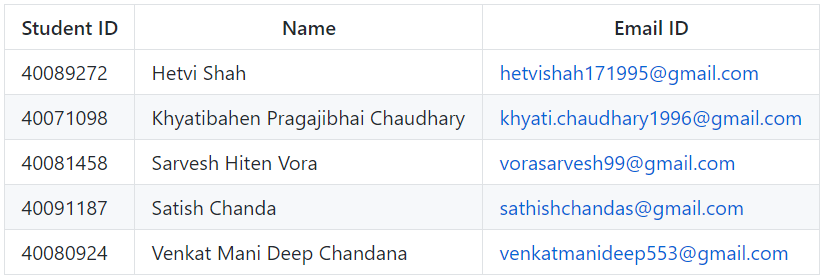
\includegraphics[scale = 1.0]{Team.png}
%
\includegraphics{GinaCody.jpg}
\end{center}

\vfill
\centerline{\textbf{\large Replication Package:} \hspace{5mm}  \large \href{https://github.com/ZenDranZer/SOEN6611}{SOEN 6611 GitHub repository} \\ }
\vfill

\centerline{April 10, 2020}
\end{titlepage}
\maketitle
\thispagestyle{plain}
\pagestyle{plain}
%%%%%%%%%%%%%%%%%%%%%%%%%%%%%%%%%%%%%%%%%%%%%%%%%%%%%%%%%%%%%%%%%%%%%%%%%%%%%%%%
\begin{abstract}
This report states various different metrics, how to calculate them and what is the correlation among them. Metrics such as Branch coverage, Statement coverage, Mutation testing, Cyclomatic complexity, Software Science Efforts, knots and Post-release defect density are identified. The data for the calculation of metrics from different projects were obtained using different tools such as CLOC, SciTool Understand. The Spearman coefficient is calculated between different metrics with the data collected from tools to determine the correlation among them.
\end{abstract}
\textit{
\textbf{Keywords---CLOC, PIT, McCabe, Post-release Defect Density, Coverage, Mutation testing, Software Science Efforts, Knots, JaCoCo, SciTools Understand, KLOC}
\newline
\textbf{Abbreviations--- CLOC: Count Lines of Code, JaCoCo: Java Code Coverage, PRDD: Post Release Defect Density, KLOC:  thousand lines of code, A.C.: Apache.Commons.}}
%%%%%%%%%%%%%%%%%%%%%%%%%%%%%%%%%%%%%%%%%%%%%%%%%%%%%%%%%%%%%%%%%%%%%%%%%%%%%%%%
\section{Introduction}
This report demonstrates the correlation among six different metrics that were calculated for four different projects using various tools. The six metrics calculated are Statement coverage, Branch coverage, Cyclomatic complexity, Mutation Score, Software Science Efforts, Knots and Post-release defect density using different tools such as EclEmma, Pit, Scitools Understand and CLOC. Metrics such as statement and branch coverage help us recognize code coverage. Mutation testing helps us to improve the test suite adequacy in terms of accuracy to detect bugs in the system. Code coverage analysis is the process of finding snippets of a program not detected by a set of test cases, which result in a quantitative measure of code coverage, which depicts code quality. Mutation Testing is when we mutate certain snippets in the source code and check if the test cases are able to find the errors, these tests can be used to improve our test cases. Cyclomatic complexity is a quantitative measure of the number of linearly independent paths through the source code. Cyclomatic complexity can be used as a benchmark to compare two different source code. Software science efforts and knots, both aims to calculate maintenance effort in terms of efforts require to understand the code \& maintain it and lastly, Post-release defect density helps us calculate the software quality by calculating the bugs and the source lines of code.\\
Here we perform a correlation among all the mentioned metrics. Specifically, 1) Correlation between code coverage metrics with Mutation testing helps us recognize test suite effectiveness. 2) Correlation between code coverage metrics with cyclomatic complexity help us to find the complexities of code which help us to improve the code quality. 3) Correlation between code coverage metrics with post-release defect density helps to find the quality of the software based on the bug report and complexity. 4)Correlation between maintenance efforts and post-release defect density is needed to check whether high maintainability causes high number of defects and vice versa.

\section{Project \& Metric Identification}
This section is dedicated to describing all projects which are used for the analysis and to describe different metrics to be calculated on those projects.
\subsection{Project Identification}

\subsubsection{Apache Commons Collections}
The Apache Commons Collections is one of the Collections Frameworks which is an increment to the earlier versions to include various data structures that help us in faster development of Java applications.It is one of the standards for collection handling in java. The Java collections are built on JDK classes by providing new interfaces, implementation, and utilities.\cite{projectcollection}\\
Project Link: \href{http://commons.apache.org/proper/commons-collections/}{Apache Commons.Collections project}\cite{projectcollection}  \\
Source code: \href{http://github.com/apache/commons-collections/}{Apache Commons.collections Github repository}\cite{projectcollectiongit}
\\
\subsubsection{Apache Commons Configuration}
The Commons Configuration software library provides a generic configuration interface which enables a Java application to read configuration data from a variety of sources. Commons Configuration provides typed access to single, and multi-valued configuration parameters. Configuration objects are created using configuration builders.\cite{projectconfiguration}\\
Project Link: \href{http://commons.apache.org/proper/commons-configuration/}{Apache Commons.Configuration project}\cite{projectconfiguration}  \\
Source code: \href{http://github.com/apache/commons-configuration/}{Apache Commons.configuration Github repository}\cite{projectconfigurationgit}
\\
\subsubsection{Apache Commons Math:}
The Apache Commons Math is a self-contained mathematics and statistics library that solves the most common problems in a java program which are not included in Java programming language or Commons Lang.\cite{projectmath}\\
Project Link: \href{http://commons.apache.org/proper/commons-math/}{Apache Commons.Math project}\cite{projectmath}  \\
Source code: \href{http://github.com/apache/commons-math/}{Apache Commons.Math Github repository}\cite{projectmathgit}
\\
\subsubsection{Apache Commons Lang:}
Lang provides helper utilities for the java.lang API, notably String manipulation methods, basic numerical methods, object reflection, concurrency, creation and serialization, and System properties. Additionally, it contains basic enhancements to java.util.Date and a series of utilities dedicated to help with building methods, such as hashCode, toString,and equals.\cite{projectlang}\\
Project Link: \href{http://commons.apache.org/proper/commons-lang/}{Apache Commons.Lang project}\cite{projectlang}  \\
Source code: \href{http://github.com/apache/commons-lang/}{Apache Commons.Lang Github repository}\cite{projectlanggit}

\begin{table}[H]
    \centering
    \resizebox{\columnwidth}{!}{
    \begin{tabular}{|c|c|c|}
    \hline 
    Project & Version & SLOC \\
    \hline 
    Apache Commons Lang & 3.3.9 & 9.6K \\
    \hline 
    Apache Commons Collections & 4.4.4 & 132K \\
    \hline 
    Apache Commons Configuration & 2.2.7 & 847K \\
    \hline 
    Apache Commons Math & 3.6.1 & 186K \\
    \hline 
    \end{tabular}
    }
\end{table}

\subsection{Metric Identification}
\subsubsection{Statement Coverage} Statement coverage is a white-box testing approach. It is also known as Line coverage. It is used to measure and calculate the number of executable statements in a program. It
is also used to check the quality of a program. Every code block is executed in statement
coverage.
\small\[Statement Coverage = \dfrac {Number of executed statements} {Total number of statements}\]
\\
\subsubsection{Branch Coverage} Branch coverage is also known as decision coverage. It covers all the edges and measures every branch in the program and fraction of independent code segments. It
also helps us to find out which sections of code don't have any branches.
\small\[Branch Coverage =\dfrac{Number of executed branches}{Total number of branches}\]
\subsubsection{Mutation Score} Mutation testing is a method of testing where we change certain statements in the
source code and check if the test cases can find errors. It is a type of White Box Testing
which is mainly used for Unit Testing.
The importance of mutation testing is, it helps to understand how well our code could
handle the faults in the program, A mutation is nothing but a small change in the
statement of the code.
Mutation testing is usually very time consuming, so we generally use a set of
automation tools like Stryker, PIT Testing, etc.
\small\[Mutation Score = \dfrac{Killed Mutants}{Total number of Mutants}*100\]
\small\[ Total no. of mutants = \dfrac{Number of mutants}{faults introduced into the code}\]
where, Number of mutants that are Identified
by the code.
Mutation testing is extremely costly and time-consuming since there are many mutant programs that need to be generated. testing cannot be done without an automation tool. Each mutation will have the same number of test cases as that of the original program. So, a large number of mutant programs may need to be tested against the original test suite.As this method involves source code changes, it is not at all applicable for Black Box Testing.
\\
\subsubsection{Cyclomatic Complexity} Cyclomatic complexity is a software metric used to indicate the complexity of the given
software by calculating the independent paths through your source code structure.
Path testing helps us to cover all the statements at least once in the program testing
period. It checks each linearly independent path which mean the total number of test
cases is equal to the cyclomatic complexity of the program.
\[McCabe(CC) = E-N+2P\]
where, $E$ = The number of edges of the graph.
$N$ = The number of nodes of the graph.
$P$ = The number of connected components.
\\
\subsubsection{Software Science Efforts}
It is an estimation of programming effort based on the number of operators and operands. It is a combination of other Software Science metrics.To calculate the Software Science Effort, we need various parameters.\\
Number of distinct operators($D$) like if, while, $\leq$, etc.\\
Number of distinct operands($E$) like variables, constants, etc.\\
Total occurrence of operators($F$).\\
Total occurrence of operands($G$).\\
Vocabulary,\[K = D + E\]
Observed length, \[L = F + G\]
The complete volume, \[V = L \times \log_2(K)\]
The Difficulty, \[D' = \frac{D \times G}{2E}\]
Software Science Effort, \[E = V \times D'\]
Algorithm: Scan the whole module code to compute parameters and perform calculations. Hypothesis: Maintainability should decrease as the effort increases.\\
But in our project, it was really difficult to obtain the number of distinct operators and operands or to find a tool that does the job done. Therefore we changed our software maintenance metric to Knots\cite{woodward1979measure}\cite{frappier1994software}.\\
\textbf{Knots:} The number of crossing lines in a control flow graph. It is used to evaluate the structure of the module. The high number of knots, the less maintainable and understandable the project is\cite{woodward1979measure}\cite{frappier1994software}.
First, we need to define the line numbers for the module from the start till the end. Any hope from line number x to line number y is represented by $(x,y)$. Let’s assume there exists two jumps in the module, $(i,k)$ and $(j,l)$. Without loss of generality, there exist a knot if and only if,
\[min(i,k) \leq min(j,l) \leq max(i,k) \leq max(j,l)\]
In our implementation we have used SciTools Understand to evaluate knots. For a particular version of a particular project, we have calculated the total number of knots for simplicity and compared them\cite{conte1986software}\cite{frappier1994software}.
\\
\subsubsection{Post-release defect density:}
It measures the compactness of defects in an application. Post-release defect density is a quality indicator for product quality. It is defined as the number of defects confirmed in software during a specific period of operation or development divided by the size of the software.
\[Defect density = \frac{Number of confirmed defects}{KLOC}\]

\section{Tools and Metric calculations:}
\subsection{Tools Identification}

\subsubsection{JaCoCo} JaCoCo is a free code coverage tool for java.
It Gives the code coverage analysis of line, methods, branches and cyclomatic complexity.
Various format of the report can be generated like HTML, CSV, XML, EXEC
Integrated JaCoCo with Maven-plugin for our project.Reasons to prefer JaCoCo is,
\begin{itemize}
  \item JaCoCo can be integrated in various IDEs such as Eclipse or Android Studio by installing a simple plugin.
  \item Simple and informative report format.
  \item The report will also highlight the lines of instructions that have not been called and/or have low code coverage.
\end{itemize}
\smallskip
\subsubsection{PIT}
PIT runs your unit tests against automatically modified versions of your application code. 
When the application code changes, it should produce different results and cause the unit tests to fail. \cite{pit}
If a unit test does not fail in this situation, it may indicate an issue with the test suite.
Reasons to prefer this tool are,\cite{pit} \cite{pitinfo}
\begin{itemize}
  \item It is a powerful approach to attain high coverage of the source program.
  \item Mutation testing brings a good level of error detection to the software developer.
  \item This method uncovers ambiguities in the source code and has the capacity to detect all the faults in the program.
  \item Customers are benefited from this testing by getting a most reliable and stable system.
\end{itemize}
\smallskip
\subsubsection{CLOC}
CLOC is used to count lines of code in the program.It computes differences of, physical lines of source code in the given files and determine a total number of lines of code in the project. Reasons to prefer this tool are, \cite{cloc}
\begin{itemize}
    \item Well maintained open-source tool
    \item Compare lines of code between versions
    \item Allows results from multiple runs to be summed together by language and by the project.
    \item Handles file and directory names with spaces and other unusual characters.
    \item Support various programming languages and OS
\end{itemize}

\subsubsection{SciTools Understand}
Understand is a customizable integrated development environment (IDE) that enables static code analysis through an array of visuals, documentation, and metric tools. Understand provides tools for metrics and reports, standards testing, documentation, searching, graphing, and code knowledge. It is capable of analyzing projects with millions of lines of code and works with code bases written in multiple languages. Reason to choose this application is that this application is simple and it does not require to build the whole project. We can simply feed the project to the application and it will dump the output.
\begin{itemize}
    \item Generate a report for our selected metric(Knots)
    \item Simple to learn and use 
\end{itemize}
\begin{table}[H]
    \centering
    \resizebox{.7\columnwidth}{!}{%
    \begin{tabular}{|c|c|}
    \hline
    Tool & Version \\
    \hline
    EclEmma JaCoCo & 8.5\\
    \hline
    PIT & 1.5\\
    \hline
    CLOC & 1.84\\
    \hline
    SciTools Understand & 5.1.1\\
    \hline
    \end{tabular}
    }
\end{table}



\subsection{Metric Calculation}
\medskip
\subsubsection{ Calculating Statement Coverage, Branch Coverage and McCabe Complexity(CC) }
Code coverage and McCabe Complexity(CC) is collected by using a specialized tool JaCoCo and run a full set of automated tests of the project. A tool gave us the list of classes with its count of lines and branches that is executed and Complexity it covered. Using JaCoCo in all selected project was quite simple with some interesting challenges.
\\JaCoCo Steps:\cite{jacocoplugin}
    \begin{enumerate}[i]
      \item Import project using maven
      \item Add  the jacoco plugin into the pom file of java project.
\begin{verbatim} 
  <plugin>
    <groupId>org.jacoco</groupId>
    <artifactId>jacoco-maven-plugin
    </artifactId>
    <reportSets>
      <reportSet>
        <reports>
          <report>report</report>
        </reports>
      </reportSet>
    </reportSets>
  </plugin>
\end{verbatim}
      \item Run the test cases
      \item Execute mvn clean install and make sure it successfully build.
      \item Execute mvn test and mvn report
      \item In the target folder , different jacoco file is generated with .html , .xml , and we are using .csv extension shows the class-wise Statement, Branch and Code Complexity coverage for the project.
    \end{enumerate}
\smallskip

\subsubsection{ Calculating Mutation Score}
We used Mutation testing tool PIT to generate a large number of mutants and run the program’s test suite on each one. If the test suite fails when it is run on a given mutant, Tool report says that the suite kills that mutant.
If a mutant is not killed by a test suite, The tool report says that mutant lived.
The quality of tests can be gauged from the percentage of mutations killed.
Moreover, PIT runs your unit tests against automatically modified versions of your application code. 
When the application code changes, it should produce different results and cause the unit tests to fail. \cite{pit}
If a unit test does not fail in this situation, it may indicate an issue with the test suite. Using PIT plugin was kind of similar process as JaCoCo.
\\PIT Steps:
  \begin{enumerate}[i]
    \item Copy the plugin into the pom file of your java project.
\begin{verbatim} 
<plugin> 
  <groupId> org.pitest </groupId> 
	  <artifactId> pitest-maven </artifactId> 
    	<version> LATEST </version> 
    		 <configuration> 
    		    <outputFormats> 
            				<param> HTML </param> 
            				<param> CSV </param> 
    			    </outputFormats> 
    		</configuration> 
</plugin>
\end{verbatim}
    \item Execute \textit{mvn clean install}
    \item Execute \textit{mvn org.pitest:pitest-maven:mutationCoverage -X}
    \item A \textit{ .csv} file is create showing various mutation score of every mutation test that has been applied to the project.
    \item Execute the \textit{ClassMutationScore.py} generator to generate class wise mutation score.
    \item Calculate \textit{Mutation Score}.
  \end{enumerate}
\smallskip

\subsubsection{Calculating Knots}
Scitools Understnad is used for various metrics like 
\begin{enumerate}[i]
    \item Register and download a trial version of the SciTools Understand by \href{https://scitools.com/trial-download-3/}{clicking here}\cite{scitoolUnderstnad}.
    \item Click on the downloaded .exe file and install Understand and start evaluation.
    \item Create a new project File $\rightarrow$ New 	$\rightarrow$ Project.
    \item Specify the project directory and click on create project.
    \item To generate Knots report, Click on Metrics 	$\rightarrow$ Export metrics.
    \item Select Knots checkbox 	$\rightarrow$ Export It will export a .csv file to the specified destination.
\end{enumerate}

\subsubsection{Calculating CLOC}
Depending your operating system, one of installation methods may require to install CLOC\cite{cloc}.\\
Installation and Configuration of CLOC:\\
\textit{cloc-1.84.exe [options] [file(s)/dir(s)/git hash(es)]} \\
Count physical lines of source code and comments in the given files (maybe archives such as compressed tarballs or zip files) and/or recursively below the given directories or git commit hashes. \\
Example: cloc src/ include/ main.c \\
cloc-1.84.exe --help shows full documentation on the options. \href{ https://github.com/AlDanial/cloc}{CLOC} has numerous examples and more information.
\medskip

\subsection{Understanding data collection}
Using the above mentioned tools, various metrics are calculated and the required data is been collected for five versions of each project.
As it is observed from collected data is not equally distributed. To study their correlation and gather more observations, we have used python with Jupyter notebooks.
Given graphs shows all metrics results for latest version of each selected project.

\begin{figure}[H]
    \centering
    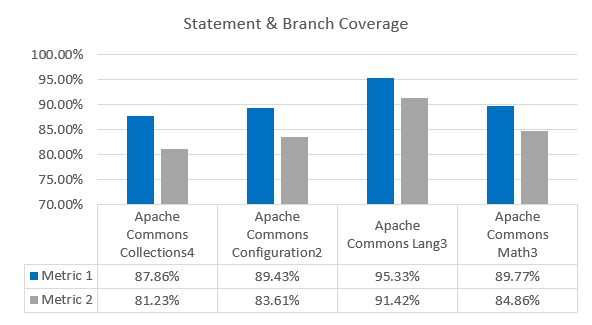
\includegraphics[scale=0.7]{Statement_Branch_analysis.PNG} %%% Metric 1 and 2 %%%
    \caption{Bar graph to depict Statement and Branch coverage for each project for their latest version.}
     \vspace{0.00mm}
    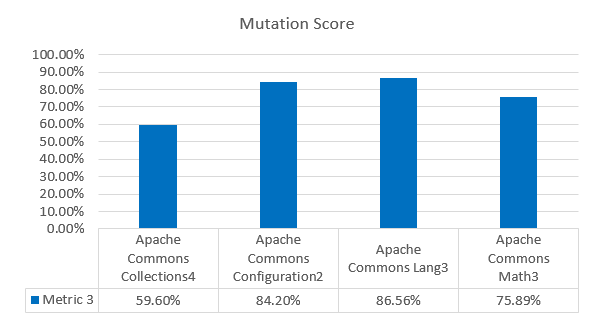
\includegraphics[scale=0.7]{Mutation_Score_analysis.PNG} %%% Metric 3 %%%
    \caption{Bar graph to depict mutation score for each project for their latest version.}
    \vspace{0.00mm}
    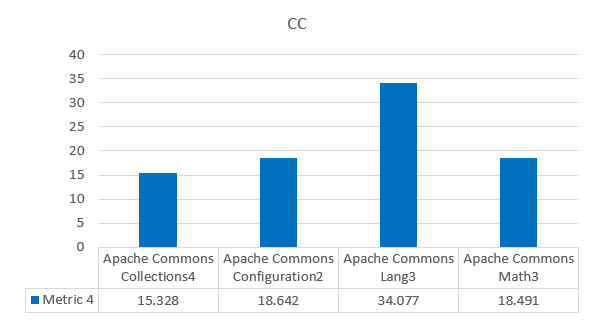
\includegraphics[scale=0.7]{Cyclomatic_Complexity_analysis.PNG} %%% Metric 4 %%%
    \caption{Bar graph to depict cyclomatic complexity for each project for their latest version.}
     \vspace{0.00mm}
    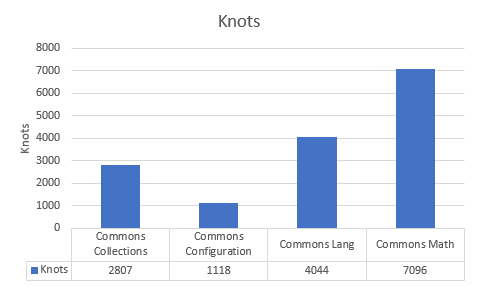
\includegraphics[scale=0.7]{knots_analysis.png} %%% Metric 5 %%%
    \caption{Bar graph to depict total number of knots for each project for their latest version.}
\end{figure}
 \begin{figure}[H]
    \centering
     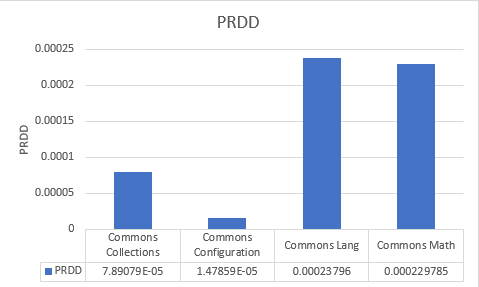
\includegraphics[scale=0.7]{PRDD_analysis.png}%%% Metric 6 %%%
    \caption{Bar graph to depict post-release defect density for each project for their latest version.}
 \end{figure}
 
\section{Metric Correlation}

\subsubsection{Correlation among Metric 1,2 with Metric 3 }
Code coverage measures the code covers by test cases and mutation score measures the fault tolerance of test cases.After performing correlation on class level data for Statement coverage, Branch coverage and Mutation score, our analysis shows they have positive correlation and as high code coverage is, high test suite effectiveness we received. \\However, We collected data for each project resulting all class level information. To study correlation, we performed some cleaning and formatting of CSV files collected by Jococo and PIT, using various Python libraries. The preprocessing of these files was a quite challenging process. Finally, \textit{spearmanr} from \textit{scipy} used to collect correlation between metrics.
\begin{figure}[H]
    \centering
     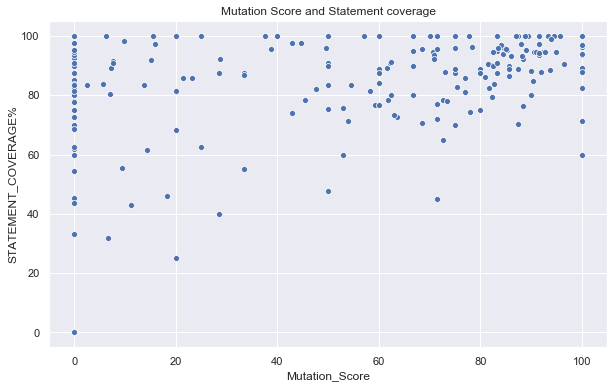
\includegraphics[scale=0.40]{metric3 vs 1 commons-collections.png}%%% Metric 1_3 %%%
     \\ 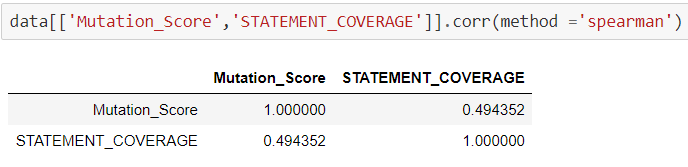
\includegraphics[scale=0.60]{metric3 vs 1 commons-collections_spearmanr.png} %%% Metric 1_3%%%
    \caption{Graph to depict Mutation Score correlation with Statement Coverage{\footnotesize[A.C.Collections]}}
\end{figure}
\begin{figure}[H]
   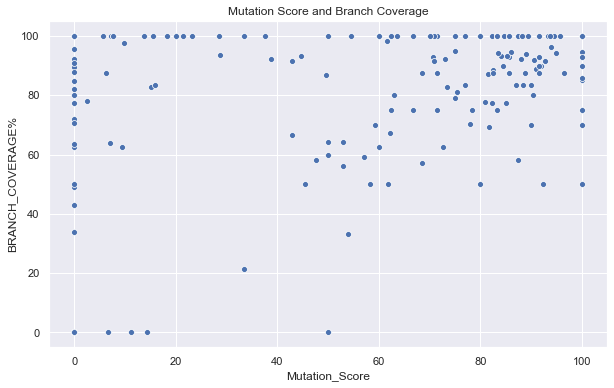
\includegraphics[scale=0.45]{metric3 vs 2 commons-collections.png}%%% Metric 2_3%%%
   \\ 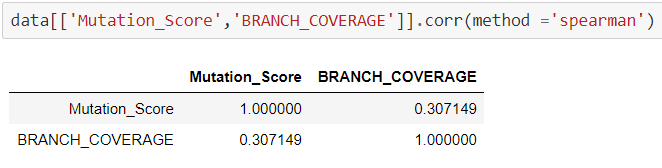
\includegraphics[scale=0.70]{metric3 vs 2 commons-collections_spearmanr.png} %%% Metric 2_3%%%
    \caption{Graph to depict Mutation Score correlation with Branch Coverage{\footnotesize[A.C.Collections]}}
 \end{figure}
\smallskip

\subsubsection{Correlation among Metric 1,2 with Metric 4 }
We assume more code coverage require more test case development and increasing code complexity made this task tough. We performed this analysis on class level for all projects with their five different versions.\\Moreover, it does not directly provide statement, branch coverage. So we have to use some formulas to format the data. for example \[ Statement coverage = \dfrac{LineCovered}{LineCovered + LineMissed}*100\]
\begin{figure}[H]
    \centering
     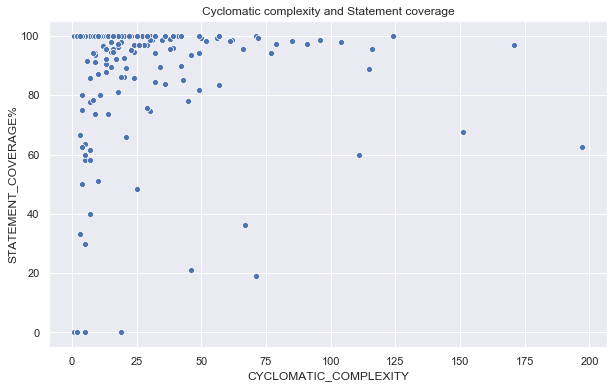
\includegraphics[scale=0.40]{metric4 vs 1 commons-configuration.png}%%% Metric 1_4 %%%
     \\ 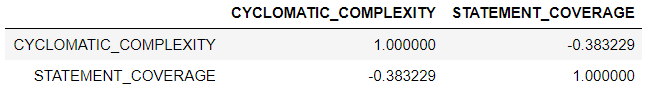
\includegraphics[scale=0.60]{metric4 vs 1 commons-config_spearmanr.png} %%% Metric 1_4%%%
    \caption{Graph to depict Cyclomatic Complexity correlation with Statement Coverage{\footnotesize[A.C.Configuration]}}
\end{figure}
The result and analysis tells that it has some inverse relation and thus we found negative for Statement coverage to McCabe complexity and Branch coverage to McCabe Complexity. We used Jacoco report as data source to perform correlation analysis.
\begin{figure}[H]
   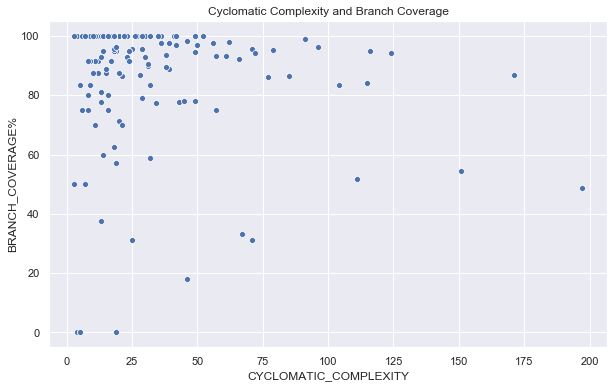
\includegraphics[scale=0.40]{metric4 vs 2 commons-configuration.png}%%% Metric 2_4%%%
   \\ 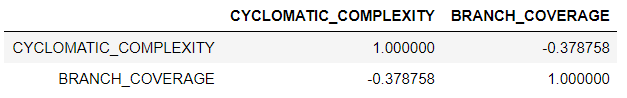
\includegraphics[scale=0.60]{metric4 vs 2 commons-config_spearmanr.png} %%% Metric 2_4%%%
    \caption{Graph to depict Cyclomatic Complexity correlation with Branch Coverage{\footnotesize[A.C.Configuration]}}
 \end{figure}
Overall, we assume that class with high complexity will have lower test coverage for Statement and Branch coverage.
\smallskip

\subsubsection{Correlation among Metric 1,2 with Metric 6 }
Comparison between Code coverage and Defect Density, required data of each project at version level. We collected five versions of each project, processed Jacoco \textit{CSV} files for code coverage and generate one excel file for each project with all version level data of Defect density.
\begin{figure}[H]
    \centering
     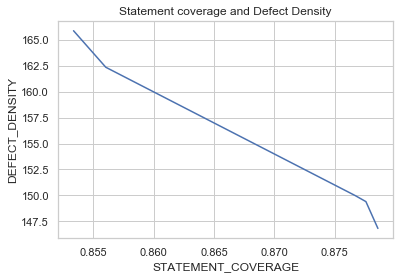
\includegraphics[scale=0.60]{metric1 vs 6 commons-collections.png}%%% Metric 1_6 %%%
     \\ 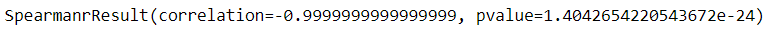
\includegraphics[scale=0.55]{metric1 vs 6 commons-collections_spearmanr.png} %%% Metric 1_6%%%
    \caption{Graph to depict post release defect density correlation with Statement Coverage{\footnotesize[A.C.Collections]}}
 \end{figure}
As observed, correlation varies from positive to negative values. Statement Coverage and Branch Coverage both have most of negative correlation with Defect density. Thus, We can conclude our assumption as high code coverage results in lowering the defects in the system. 
\begin{figure}[H]
    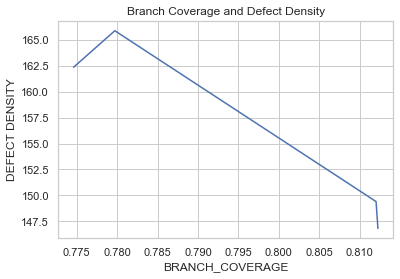
\includegraphics[scale=0.60]{metric2 vs 6 commons-collections.png}%%% Metric 2_6 %%%
    \\ 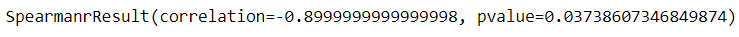
\includegraphics[scale=0.60]{metric2 vs 6 commons-collections_spearmanr.png} %%% Metric 2_6%%%
    \caption{Graph to depict post release defect density correlation with Branch Coverage{\footnotesize[A.C.Collections]}}
 \end{figure}
\smallskip

\subsubsection{Correlation among Metric 5 with Metric 6 }
Correlation between Knots and Defect Density required version level information for each project. We calculated metric 5 and metric 6 on five versions of each project. The defect density was calculated by counting number of bugs raised in project's issue tracking repository. In metric 5, The high number of knots, the less maintainable and understandable the project is.
\begin{figure}[H]
    \centering
     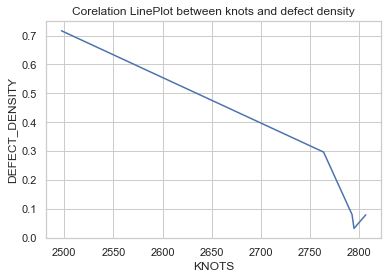
\includegraphics[scale=0.60]{metric5 vs 6 commons-collections.png}%%% Metric 5_6 %%%
   \\  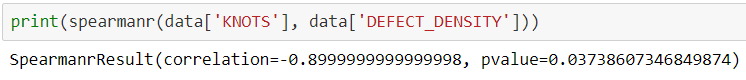
\includegraphics[scale=0.55]{metric5 vs 6 commons-collections_spearmanr.png} %%% Metric 5_6%%%
    \caption{Graph to depict post release defect density correlation with knots{\footnotesize[A.C.Collections]}}
 \end{figure}
We have performed correlation using \textit{Spearmanr}, after our deep analysis of each metric. We found out that all but one of the projects had different result. \\We can observe that A.C.collections, A.C.lang and A.C.configuration show an inverse correlation. An inverse correlation is when the number of knots increases, the defect density decreases. We can understand that having a lot of knots makes the code really difficult to track and maintain therefore, we might skip many bugs and the defect density decreases. Whereas the A.C.math depicted different results as it was the only positive correlation and we can understand that as the versions are updated, we may acquire more knots but the defect density is increases due to its defect identification system.

\section{Related work}
This paper comprises the examination of four open-source Java projects and measures
the software quality and maintenance efforts. The paper studied various metrics for ascertaining code coverage and quality. Research and observation shows express that
there is a low to direct connection amongst coverage and effectiveness when the quantity of
experiments in the suite is controlled for. that more grounded types of coverage don't give more noteworthy knowledge into the adequacy of the suite. Their outcomes propose that
coverage, while helpful for distinguishing under-tested pieces of a program, should not be
utilized as a quality objective since it's not a good indicator of test suite effectiveness.
\\ In metric 6, The developers gather genuine
bugs logged in the issue tracking system after the arrival of the product and investigate the
connections between code inclusion and these bugs.
They additionally gather different metrics, for example, cyclomatic complexity and lines of code,
which are utilized to standardize the number of bugs and coverage to correspond with different
measurements just as utilize these metrics in regression analysis. Their outcomes show that
coverage has an inconsequential relationship with the number of bugs that are found after the
release of the software at the project level and no such connection at the document level.
\medskip

\section{Future work}
We can identify future work to test the metrics on significantly large projects or projects which are in the build process in order to identify structural integrity and other aspects of software at the early stage to avoid refactoring. To be accurate and precise in our metric calculation, we may need few more projects and may consider more version of them. In this study we have only considered the java project, but we can define our metrics for other programming languages as well. Apart from that we have detected few quality attributes like code coverage, maintainability and testability but we may study different quality attributes such as usability by performing operations on the UI, availability by performing denial of service attack or security by performing various penetration testing.
\medskip
\section{Conclusion}
This Paper studies various metrics such as Statement Coverage, Branch Coverage, Mutation Score, Cyclomatic Complexity, Knots and Post Release Defect Density. After analyzing five versions of selected projects, research concluded with below statements,
\\The selection process for metric 5 software maintenance metric was really weak. The Software Science Efforts metric is really difficult to calculate and we do not recommend to use Software Science Efforts for it. However if there exist a tool to calculate it then one must consider Software Science Efforts. The knots on the other hand is easy to implement and understandable metric for the software maintenance.
\\Code coverage has an inverse relation with McCabe Complexity. Whereas they have positive and direct relation with Test suite effectiveness. On other side, Code coverage metric and defect density share inverse correlation, where less the code coverage result in high defects with each new release.
\\Correlating Knots with Defect Density gives quite different results for different projects. For Commons-Math, it reacts with a positive result. However for other projects, it gives inverse relations. This difference might be possible because of bug fixes in new versions or due to its defect identification system.
\medskip



\balance
\bibliographystyle{ieeetr}
\bibliography{bibliography}


\clearpage

\end{document}